\documentclass{article}
\usepackage[T1]{fontenc}
\usepackage{lmodern}
\usepackage{graphicx}
\usepackage{amsmath,amssymb}
\usepackage[a4paper,margin=2cm]{geometry}
\usepackage[absolute,overlay]{textpos}
\setlength{\TPHorizModule}{1mm}
\setlength{\TPVertModule}{1mm}
\usepackage[indonesian]{babel}
\usepackage{hyperref}
\setlength{\emergencystretch}{2em}
% unit: Halaman 24

\begin{document}

% === Halaman 24 (llm) ===

\section*{Steganografi dan Terorisme}

\begin{itemize}
    \item Ilmu steganografi mendadak naik daun ketika pasca 11 September 2001 pihak FBI menuding Al-Qaidah menggunakan steganografi untuk menyisipkan pesan rahasia melalui video atau gambar yang mereka rilis secara teratur di Internet.
\end{itemize}

\vspace{10mm}

% deskripsi: Foto gedung World Trade Center yang terbakar setelah serangan 11 September.
% bbox normalisasi: [0.1380, 0.5010, 0.4140, 0.8860]
\begin{textblock*}{57.96mm}(28.98mm,148.80mm)
\noindent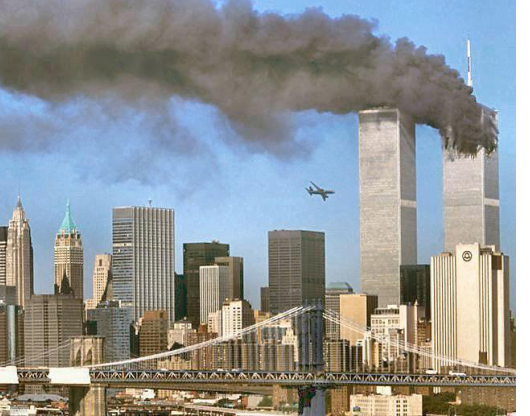
\includegraphics[width=57.96mm,height=114.34mm]{../../images/llm/page_024_img_01.png}%
\end{textblock*}

% deskripsi: Screenshot cuplikan video yang menampilkan teks Arab dan bendera Al-Qaeda.
% bbox normalisasi: [0.5360, 0.5010, 0.7630, 0.8930]
\begin{textblock*}{47.67mm}(112.56mm,148.80mm)
\noindent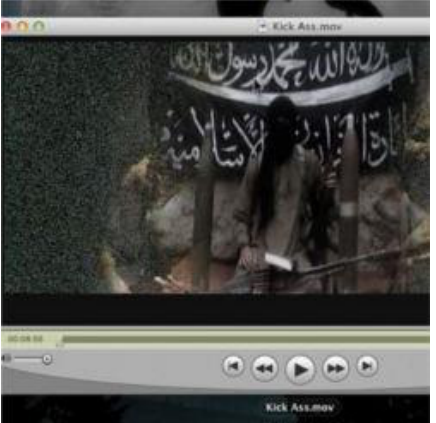
\includegraphics[width=47.67mm,height=116.42mm]{../../images/llm/page_024_img_02.png}%
\end{textblock*}

\end{document}
